\section{ 悲しいほど貴方が好き}

\large{

\ruby{気}{き}がついたら \ruby{恋}{こい}しかった

\ruby{悲}{かな}しい\ruby{出来事}{ニュース} あふれる\ruby{街}{まち}で

\ruby{貴方}{あなた}の\ruby{声}{こえ}が\ruby{聴}{き}けない\ruby{日}{ひ}は

\ruby{私}{わたし}の すべてが\ruby{止}{と}まる
\\

\parpic[r]{
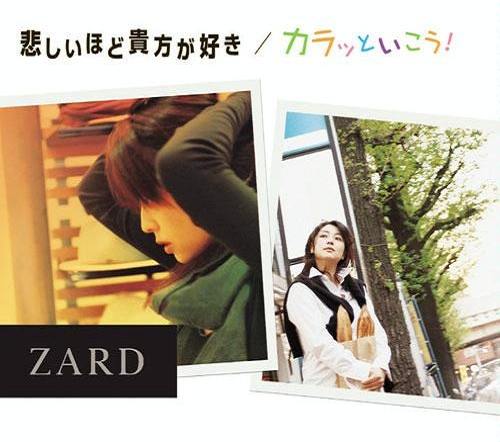
\includegraphics[width=0.4\textwidth]{S41.jpg}}

\ruby{悲}{かな}しいほど \ruby{貴方}{あなた}がすきで

\ruby{恋}{こい}しすぎると「\ruby{何故}{なぜ}なの?」

こんなにも\ruby{苦}{くる}しい…

\ruby{勇気}{ゆうき}を\ruby{持}{も}って \ruby{新}{あたら}しい\ruby{世界}{せかい}の

\ruby{扉}{とびら} \ruby{開}{あ}け\ruby{放}{はな}とう

\ruby{貴方}{あなた}が \ruby{私}{わたし}の\ruby{心}{こころ}を

\ruby{朝焼}{あさや}けに\ruby{染}{そ}めた

So. I'll make it with you
\\

\ruby{空}{そら}を\ruby{飛}{と}ぶ \ruby{鳥}{とり}のように

\ruby{大空}{おおぞら}を \ruby{自由}{じゆう}に\ruby{飛}{と}びたい

\ruby{貴方}{あなた}がふさぎ\ruby{込}{こ}み うつむく\ruby{日}{ひ}は

\ruby{私}{わたし}が そっと \ruby{照}{て}らしてあげたい
\\

\ruby{悲}{かな}しいほど \ruby{貴方}{あなた}がすきで

\ruby{恋}{こい}は\ruby{綱引}{つなひ}きね

どんどん\ruby{貴方}{あなた}へ \ruby{引}{ひ}っ\ruby{張}{ぱ}られていくみたい

また\ruby{明日}{あした}は \ruby{逢}{あ}えるのかな

どうしていいか \ruby{分}{わ}からないくらい

\ruby{貴方}{あなた}が \ruby{私}{わたし}の\ruby{心}{こころ}を

\ruby{夕焼}{ゆうや}けに \ruby{染}{そ}めた
\\

\ruby{瞳}{ひとみ}に \ruby{星}{ほし}\ruby{降}{ふ}る キャンバス

\ruby{未来}{みらい}を\ruby{示}{しめ}している\ruby{星}{ほし}はどれ?
\\

\ruby{悲}{かな}しいほど \ruby{貴方}{あなた}がすきで

\ruby{恋}{こい}しすぎると「\ruby{何故}{なぜ}なの?」

こんなにも\ruby{苦}{くる}しい…

\ruby{勇気}{ゆうき}を\ruby{持}{も}って \ruby{新}{あたら}しい\ruby{世界}{せかい}の

\ruby{扉}{とびら} \ruby{開}{あ}け\ruby{放}{はな}とう

\ruby{貴方}{あなた}が \ruby{私}{わたし}の\ruby{心}{こころ}を

\ruby{七色}{なないろ}に\ruby{染}{そ}めた
\\

\ruby{七色}{なないろ}に\ruby{染}{そ}めた

So. I'll make it with you

}